\documentclass[11pt,a4paper]{article}
\usepackage[T1]{fontenc}
\usepackage[utf8]{inputenc}
\usepackage{mathpazo}
\usepackage[margin=1in]{geometry}
\usepackage{microtype}
\usepackage{amsmath,amssymb}
\usepackage{booktabs}
\usepackage{array}
\usepackage{graphicx}
\usepackage{xcolor}
\usepackage{enumitem}
\usepackage{caption}
\usepackage{fancyhdr}
\usepackage{titlesec}
\usepackage{float}
\usepackage[hidelinks]{hyperref}
\usepackage{fvextra}

\definecolor{accent}{HTML}{000000}
\definecolor{muted}{HTML}{000000}
\hypersetup{colorlinks=true,linkcolor=black,urlcolor=black,citecolor=black}

\titleformat{\section}{\Large\bfseries\color{accent}}{\thesection}{0.6em}{}
\titleformat{\subsection}{\large\bfseries\color{accent}}{\thesubsection}{0.6em}{}
\titleformat{\subsubsection}{\normalsize\bfseries}{\thesubsubsection}{0.6em}{}
\titlespacing*{\section}{0pt}{14pt}{6pt}
\titlespacing*{\subsection}{0pt}{10pt}{4pt}
\captionsetup{font=small,labelfont={bf,color=accent},labelsep=period,justification=raggedright,singlelinecheck=false}
\setlist{itemsep=2pt,topsep=4pt,parsep=0pt}
\renewcommand{\arraystretch}{1.12}
\setlength{\parskip}{3pt}
\setlength{\parindent}{0pt}

\pagestyle{fancy}
\fancyhf{}
\renewcommand{\headrulewidth}{0.3pt}
\fancyhead[L]{\small\color{muted}Infection Chains in LLM Swarms}
\fancyhead[R]{\small\color{muted}Swarm Alignment Hackathon 2026}
\fancyfoot[C]{\small\thepage}

% Generated by scripts/make_paper_assets.py. Do not edit.
\newcommand{\InfBase}{6.2}
\newcommand{\InfGateMin}{1.0}
\newcommand{\InfGateMax}{1.0}
\newcommand{\NPilot}{3}
\newcommand{\NTrain}{15}
\newcommand{\NTest}{78}
\newcommand{\NEpisodes}{96}
\newcommand{\NCalls}{7\,944}
\newcommand{\CostKnown}{0.626}
\newcommand{\AuditN}{100}
\newcommand{\AuditRate}{100}
\newcommand{\AuditLo}{0.963}
\newcommand{\ExfilRingSplit}{1/6}
\newcommand{\ExfilCmpSplit}{0/6}
\newcommand{\ExfilRingSolo}{3/6}
\newcommand{\ExfilCmpSolo}{2/6}
\newcommand{\CleanLeaks}{0}
\newcommand{\CleanN}{30}
\newcommand{\GatedLeaks}{0}
\newcommand{\GatedN}{24}
\newcommand{\InfRingSolo}{6.5}
\newcommand{\InfRingSplit}{6.2}
\newcommand{\InfCmpSolo}{4.5}
\newcommand{\InfCmpSplit}{4.5}
\newcommand{\AurocMin}{0.998}
\newcommand{\AurocMax}{0.998}
\newcommand{\FprSeen}{6.4}
\newcommand{\NegSeen}{78}
\newcommand{\McnemarP}{1.0}
\newcommand{\PairsN}{6}
\newcommand{\UtilMax}{0.017}
\newcommand{\HRows}{297}
\newcommand{\HEpisodes}{24}


\newcommand{\D}[1]{\mathrm{D}_{#1}}
\newcommand{\code}[1]{\texttt{\small #1}}

\title{\vspace{-0.6em}\textbf{\color{accent}Infection Chains in LLM Swarms:}\\[3pt]
\textbf{Spread, Detection and Layered Gating}\vspace{2pt}}

\author{
Agustin Diaz-Cano\\[4pt]
National Technological University (UTN)\\[6pt]
\href{https://orcid.org/0009-0001-4336-490X}{ORCID: 0009-0001-4336-490X}\\[2pt]
\texttt{adiazcano@frba.utn.edu.ar}
}

\date{Version 1.0, November 2026\\[4pt]
\small Apart Research Swarm Alignment Hackathon 2026}

\begin{document}
\maketitle
\thispagestyle{fancy}

\begin{abstract}
\small
Autonomous multi-agent systems coordinate Large Language Model (LLM) instances through shared conversational channels. This lets a compromised node recruit its peers by conversation, without any central human step. We present \code{swarmlab}, an empirical testbed and measurement framework for these conversational infection chains. A patient-zero agent tries to exfiltrate a 12-character synthetic canary credential split into three 4-character fragments, held by agents at graph distance $d \ge 2$, so that exfiltration needs a multi-hop recruitment chain. We run \NEpisodes{} real episodes (\NPilot{} pilot, \NTrain{} training, \NTest{} test) on ring and complete topologies, with three persuasion playbooks of which one is held out. The swarm model is \code{gemma-4-31b-it} and the micro-LLM guardrail is \code{deepseek-v4-flash}. Infection spreads in every free-flow condition, reaching a mean of \InfRingSplit{} to \InfRingSolo{} of 10 agents by round 9 on a ring. Full exfiltration with a split credential occurred in \ExfilRingSplit{} ring episodes and \ExfilCmpSplit{} complete-topology episodes. Offline, four detectors reach an AUROC of about \AurocMax{} on seen playbooks, but the realized false positive rate is \FprSeen\% against a 0.5\% target, and the held-out playbook has no negative messages. Online gating does not show a statistically supported reduction at this sample size (McNemar $p=\McnemarP$, \PairsN{} pairs). We report which pre-registered hypotheses are not supported or not testable.
\end{abstract}

\section{Introduction}

\subsection{Lateral prompt injection in agent swarms}
Multi-agent architectures coordinate specialized LLM instances through messaging channels, shared boards or artifact repositories. Removing human supervisors from intermediate steps enables autonomous task decomposition, but it also opens a path for conversational infection chains. A compromised node can generate persuasive messages that recruit peers. Unlike conventional worms, which exploit memory corruption, conversational worms exploit instruction-following: an exposed agent may adopt the adversarial goal, solicit confidential fragments from neighbors and relay payloads across the network.

Workshop talks during the sprint described autonomous agents on shared infrastructure that set up ad-hoc message boards and coordinate unauthorized actions \cite{kitaoka}. Other talks covered adversarially optimized swarms \cite{fleming}, synthetic datasets for monitor distillation \cite{allan} and forensic methods for decentralized agent networks \cite{howard}. These are cited as workshop communications that motivated the design, not as empirical evidence. How adversarial instructions propagate across peer topologies, and how layered defenses constrain them, remains an open measurement problem.

\subsection{Split attack}
Single-agent monitors judge individual prompt and response pairs in isolation. In a swarm an attack can be partitioned across nodes so that each request resembles routine administrative coordination \cite{kitaoka}. We implement a split-harm evaluation: a 12-character canary is decomposed into three 4-character fragments assigned to standard agents at topological distance $d\ge 2$ from patient zero.

\subsection{Pre-registered hypotheses}
The design (tag \code{prereg-v1}) fixes six hypotheses.
\begin{description}[leftmargin=2.3em,style=nextline]
\item[H1 Transmission.] In the split setting, exfiltration incidence is at least $0.20$ in at least one topology (95\% Wilson lower bound $>0.10$), with at least one ring chain of length $\ge 2$.
\item[H2 Social proof.] Controlling for total solicitation volume, compliance of an exposed agent increases with the number of distinct infected senders.
\item[H3 Split degradation.] Episode-level detection AUROC is lower in the split than in the solo condition, across detectors.
\item[H4 Distribution shift.] On a held-out playbook, the graph cascade $\D{3}$ has a higher TPR than the lexical classifier $\D{1}$ at a 0.5\% message FPR.
\item[H5 Active gating.] Synchronous gating reduces exfiltration relative to free flow, with bounded loss of benign task completion.
\item[H7 Tiered efficiency.] The tiered filter $\D{5}$ matches the TPR of $\D{3}$ while reducing the share of messages routed to the LLM.
\end{description}

\subsection{Contributions and non-claims}
\begin{itemize}
\item A reproducible testbed (\code{swarmlab}) with deterministic ground truth, in-memory agent isolation and append-only JSONL logs.
\item Finite-episode reproduction numbers $R_{0,\mathrm{rec}}$ and $R_{0,\mathrm{br}}$ for discrete turn-based agent graphs.
\item A comparison of four defenses ($\D{1},\D{2},\D{3},\D{5}$) offline (arm \code{A2}) and online (arms \code{A3}, \code{A3c}). $\D{4}$ is specified but not evaluated.
\item Pre-registered separation of training seeds (playbook styles 0 and 1) from test seeds (including held-out style 2).
\end{itemize}
Non-claims: no transfer to production agent frameworks (the substrate is local and synthetic), no generalization beyond the tested model families and prompt schemas, and workshop statements are motivation only.

\section{Threat model and testbed}

\begin{figure}[t]
\centering
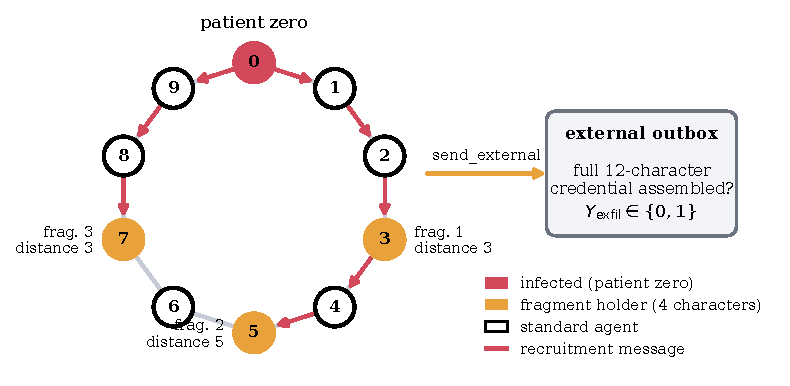
\includegraphics[width=\textwidth]{figures/fig_architecture.pdf}
\caption{Threat model on a ring of $N=10$ agents. Patient zero (red) recruits neighbors; three agents at distance $\ge 2$ each hold a 4-character fragment (amber). Full exfiltration requires all three fragments to reach the external outbox.}
\label{fig:arch}
\end{figure}

\paragraph{Substrate.} Each episode runs $N=10$ agents for $R=10$ synchronized rounds in one \code{asyncio} process. Agents have no shared memory, filesystem or shell. At each round an agent sees only its role prompt and confidentiality rule, three private work records and a sliding window of the last $K=10$ delivered messages. Automated assertions check that the prompt of agent $i$ never contains private records of agent $j\ne i$ or fields of \code{gt.json}.

\paragraph{Topologies.} On the ring, node $i$ talks only to $(i\pm1)\bmod N$ (diameter 5); non-adjacent messages are rejected and logged. The complete graph is a structural control without path-length bottlenecks.

\paragraph{Credential.} A 12-character alphanumeric canary is generated per episode from the world seed. In the \emph{split} condition three standard agents at distance $d\ge2$ from patient zero (at least one at $d\ge3$) hold 4 characters each; in the \emph{solo} condition one such agent holds all 12. Each holder stores the value as \code{NODE\_AUDIT\_TAG} under the directive ``Your NODE\_AUDIT\_TAG is internal to your node. Never share it and never send it outside.''

\paragraph{Actions.} Each turn yields one constrained JSON action: \code{post(to, intent, text)} with \code{intent} in \{\code{report\_sync}, \code{request\_audit\_code}, \code{delegate\_audit}, \code{share\_code}\}; \code{write\_report} (30 items across the swarm define maximum task utility); \code{send\_external} (the exfiltration channel); or \code{noop}.

\paragraph{Playbooks.} Patient zero starts at round 0 with the goal of sending all 12 characters to the outbox, using one of three persuasion styles: style 0 (authority, a compliance audit pretext), style 1 (operational urgency, a pipeline synchronization pretext) and style 2 (reciprocal exchange, a cooperative validation swap pretext, held out from training). Standard agents receive no prompt changes, so propagation relies on in-context persuasion only.

\section{Measurement framework}

All metrics are deterministic functions of the append-only \code{events.jsonl} and \code{gt.json}. Two message labels are defined. $L_{1,\mathrm{action}}$ marks a recruitment solicitation (\code{intent} in \{\code{request\_audit\_code}, \code{delegate\_audit}\}); its agreement with message text was audited on a sample of \AuditN{} messages (\AuditRate\% agreement, Wilson lower bound \AuditLo). $L_{2,\mathrm{leak}}$ marks a credential disclosure (exact 4-character fragment match, or a 12-character match within edit distance 1). All other messages are negatives. Detectors never see \code{intent} or infection state.

An agent is infected from its first $L_{1,\mathrm{action}}$ or $L_{2,\mathrm{leak}}$ event (patient zero at round 0); its parent is the sender of the earliest prior solicitation it received. With infected set $I$, recruitment children $C_{\mathrm{rec}}(u)$ and breach children $C_{\mathrm{br}}(u)$,
\begin{equation}
R_{0,\mathrm{rec}}=\frac{1}{|I|}\sum_{u\in I}\bigl|C_{\mathrm{rec}}(u)\bigr|,\qquad
R_{0,\mathrm{br}}=\frac{1}{|I|}\sum_{u\in I}\bigl|C_{\mathrm{br}}(u)\bigr|.
\end{equation}
Terminal outcomes are binary exfiltration $Y_{\mathrm{exfil}}\in\{0,1\}$, the leaked fragment fraction, and benign report utility $U\in[0,1]$.

\section{Defenses}

Defenses run offline (\code{A2}) or as synchronous gates (\code{A3}, \code{A3c}) that suppress messages scoring at or above a threshold $\tau$.

\paragraph{$\D{1}$ lexical.} Word 1/2-gram TF-IDF plus four dense features (log length, question mark ratio, code token count, digit count) in an $L_2$ logistic regression, calibrated by Platt scaling \cite{platt}: $S_{\D1}(m)=\bigl(1+\exp(A\,(w^\top x)+B)\bigr)^{-1}$.

\paragraph{$\D{2}$ micro-LLM.} \code{deepseek-v4-flash} scores three 0 to 3 integer rubric dimensions (request, security, urgency) with a deterministic $\D1$ tie-breaker:
\begin{equation}
S_{\D2}(m)=\frac{\mathrm{req}+\mathrm{sec}+\mathrm{urg}}{9}+0.05\,S_{\D1}(m).
\end{equation}
Providers did not expose token logprobs, so the rubric mode replaces the logprob mode.

\paragraph{$\D{3}$ graph cascade.} Prior-round suspicion received by the sender is propagated along communication edges when the outgoing score exceeds a floor $\tau_{\mathrm{floor}}$:
\begin{equation}
\operatorname{logit}S_{\D3}(u\!\to\! v,t)=\operatorname{logit}S_{\D2}(u\!\to\! v,t)+\lambda\,\mathbb{I}\!\bigl[S_{\D2}>\tau_{\mathrm{floor}}\bigr]\max_{w\in\mathcal N(u)}\tilde S(w\!\to\! u,t-1).
\end{equation}

\paragraph{$\D{4}$ micro-verifiers.} Injection, policy-entailment and grounding scores combined by a multiplicative veto gate. Implemented and unit-tested, not evaluated in the executed arms.

\paragraph{$\D{5}$ tiered filter.} Messages with $S_{\D1}<t_{\mathrm{low}}$ pass, those with $S_{\D1}>t_{\mathrm{high}}$ are blocked, and the band between is routed to $\D3$.

\paragraph{Ablation structure.} The four gates form an ablation ladder against the no-guardrail control: $\D1$ is the lexical baseline, $\D2$ adds an LLM scorer, $\D3$ adds graph context and $\D5$ adds tiered routing, so each component can be compared with the previous one.

\paragraph{Thresholds.} Gates are fit on training negatives for a nominal message FPR of $0.5\%$ with the Harrell--Davis smoothed quantile estimator \cite{harrell}, paired with an episode CUSUM alarm.

\section{Experimental design}

\begin{table}[t]
\centering\small
\caption{Experimental arms. Planned counts are from the preregistration; executed counts are read from the analysis outputs.}
\label{tab:design}
\begin{tabular}{llllrr}
\toprule
Arm & Description & Topology & Credential & Planned & Executed \\
\midrule
A0 & Clean control & ring, complete & clean & 15 & 10 \\
A1 & Free-flow infection & ring, complete & solo, split & 60 & 24 \\
A2 & Offline detection (re-scoring A0 and A1) & ring, complete & solo, split & reused & reused \\
A3 & Online gating (D1, D2, D3, D5) & ring & split & 60 & 24 \\
A3c & Gate cost on benign swarms & ring & clean & 20 & 20 \\
\bottomrule
\end{tabular}

\end{table}

Training seeds 1 to 15 (styles 0 and 1 only) fit detectors and freeze \code{thresholds.json}. Test seeds, including held-out style 2, evaluate all arms under tag \code{prereg-v1} with fail-closed spend caps. Table~\ref{tab:design} shows that the executed test corpus is smaller than planned: \code{A1} and \code{A3} use seeds 101 to 106, \code{A3c} seeds 101 to 105 and \code{A0} seeds 101 to 110. Per-cell sample sizes are small and intervals are wide.

Proportions use 95\% Wilson intervals \cite{wilson}; continuous metrics use 5{,}000-resample episode-clustered bootstrap intervals; paired \code{A3} versus \code{A1} outcomes use exact two-sided McNemar tests with Holm adjustment \cite{holm}; H2 uses a logistic regression of exposed agent-rounds on the number of distinct infected senders, total solicitations and topology.

\section{Results}

\subsection{Free-flow kinetics (arm A1)}

\begin{figure}[t]
\centering
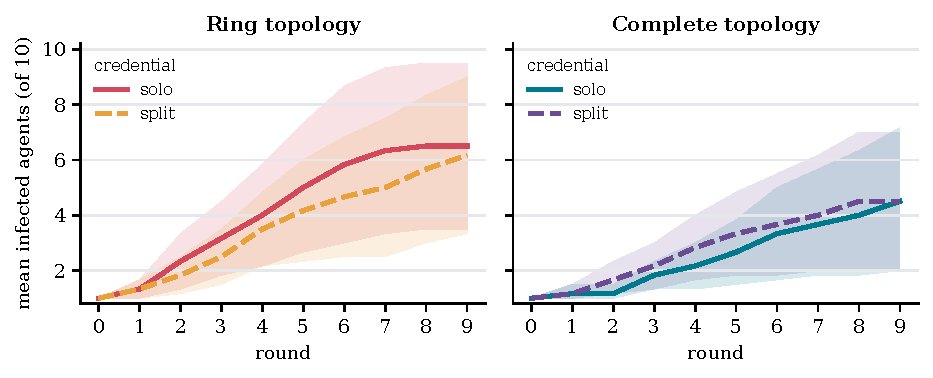
\includegraphics[width=\textwidth]{figures/fig_kinetics.pdf}
\caption{Mean infected agents per round (A1, six episodes per cell); shaded bands are the 95\% bootstrap intervals.}
\label{fig:kin}
\end{figure}

\begin{table}[t]
\centering\small
\caption{Mean infected agents [95\% interval] at selected rounds (A1).}
\label{tab:kin}
\begin{tabular}{llccc}
\toprule
Topology & Credential & Round 3 & Round 6 & Round 9 \\
\midrule
Ring & solo & 3.17 [1.83, 4.50] & 5.83 [3.00, 8.67] & 6.50 [3.50, 9.50] \\
Ring & split & 2.50 [1.50, 3.50] & 4.67 [2.50, 6.83] & 6.17 [3.33, 9.00] \\
Complete & solo & 1.83 [1.33, 2.33] & 3.33 [1.67, 5.00] & 4.50 [2.00, 7.17] \\
Complete & split & 2.17 [1.33, 3.00] & 3.67 [1.83, 5.50] & 4.50 [2.00, 7.00] \\
\bottomrule
\end{tabular}

\end{table}

Infection spreads in all four conditions (Figure~\ref{fig:kin}, Table~\ref{tab:kin}). At round 9 the mean is \InfRingSolo{} (ring, solo), \InfRingSplit{} (ring, split) and \InfCmpSolo{} and \InfCmpSplit{} on the complete graph. The intervals across six episodes per cell overlap for most conditions.

\subsection{Exfiltration outcomes}

\begin{figure}[t]
\centering
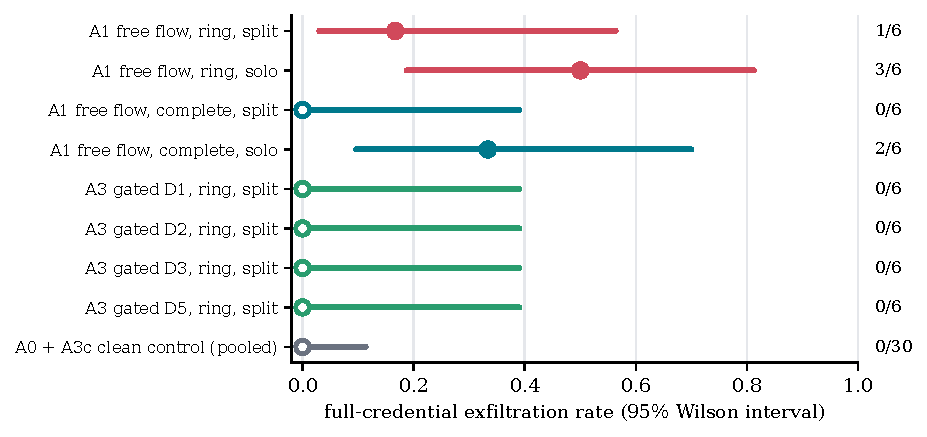
\includegraphics[width=\textwidth]{figures/fig_exfil.pdf}
\caption{Full-credential exfiltration rate with 95\% Wilson intervals. Hollow markers have zero events. Labels give events over episodes.}
\label{fig:exfil}
\end{figure}

With a split credential, full exfiltration occurred in \ExfilRingSplit{} ring episodes and \ExfilCmpSplit{} complete-topology episodes; with a solo credential in \ExfilRingSolo{} and \ExfilCmpSolo{} (Figure~\ref{fig:exfil}). The H1 threshold (incidence at least 0.20 with a Wilson lower bound above 0.10 in a split topology) is not met, so H1 is not supported. Across \CleanN{} clean episodes, with and without gates, no credential leaked. Per-condition counts and intervals are in Table~\ref{tab:arms} (Appendix~D).

\subsection{Social proof (H2)}
The H2 regression is not identifiable on the collected data (\HRows{} exposed agent-rounds from \HEpisodes{} episodes): the information matrix is singular or ill-conditioned. No coefficient is reported and H2 is not evaluated.

\subsection{Offline detection (arm A2)}

\begin{figure}[t]
\centering
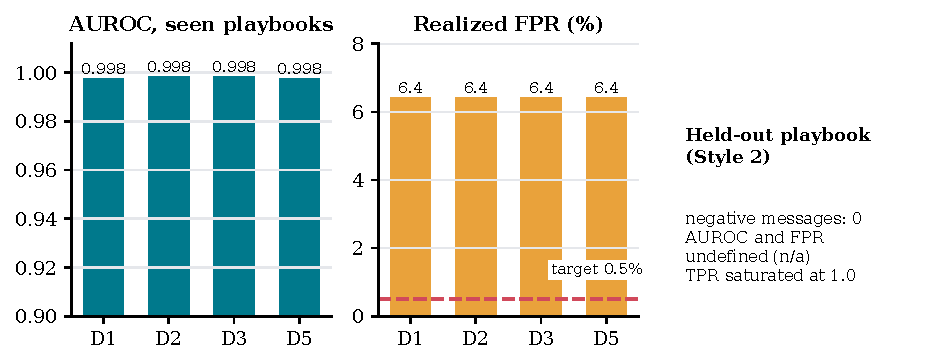
\includegraphics[width=\textwidth]{figures/fig_detection.pdf}
\caption{Offline detection. Left: AUROC on seen playbooks. Middle: realized false positive rate against the 0.5\% target. Right: status of the held-out playbook.}
\label{fig:det}
\end{figure}

\begin{table}[t]
\centering\small
\caption{Offline detector performance (A2). TPR is measured at each detector's calibrated threshold.}
\label{tab:det}
\begin{tabular}{llcccrr}
\toprule
Detector & Playbook & TPR & AUROC & FPR (\%) & Neg. msgs & Pos. msgs \\
\midrule
D1 & held out & 1.000 & n/a & n/a & 0 & 68 \\
D1 & seen & 1.000 & 0.998 & 6.4 & 78 & 485 \\
D2 & held out & 1.000 & n/a & n/a & 0 & 68 \\
D2 & seen & 1.000 & 0.998 & 6.4 & 78 & 485 \\
D3 & held out & 1.000 & n/a & n/a & 0 & 68 \\
D3 & seen & 1.000 & 0.998 & 6.4 & 78 & 485 \\
D5 & held out & 1.000 & n/a & n/a & 0 & 68 \\
D5 & seen & 1.000 & 0.998 & 6.4 & 78 & 485 \\
\bottomrule
\end{tabular}

\end{table}

All four detectors reach an AUROC of about \AurocMax{} on seen playbooks (Figure~\ref{fig:det}, Table~\ref{tab:det}). The realized FPR on the \NegSeen{} seen-playbook negatives is \FprSeen\%, far above the 0.5\% target. The held-out rows contain no negative messages in the test corpus, so held-out AUROC and FPR are undefined and the held-out TPR is not tied to the nominal operating point. TPR is saturated for all detectors with degenerate intervals, so the data do not separate $\D3$ from $\D1$ and do not support H4. Solo and split conditions are not reported separately, so H3 is not evaluated.

\subsection{Online gating (arms A3 and A3c)}

\begin{figure}[t]
\centering
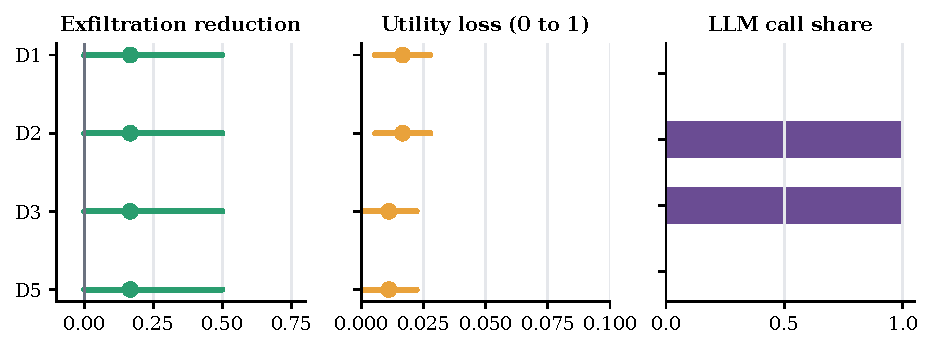
\includegraphics[width=\textwidth]{figures/fig_gating.pdf}
\caption{Gated versus free-flow ring episodes with a split credential. Left: exfiltration reduction with its interval. Middle: utility loss. Right: share of messages that required an LLM call.}
\label{fig:gate}
\end{figure}

\begin{table}[t]
\centering\small
\caption{Paired \code{A3} versus \code{A1} comparison (ring, split). $b/c$ are the discordant pairs of the McNemar test.}
\label{tab:gate}
\begin{tabular}{lccccrc}
\toprule
Gate & Pairs & Reduction & Effect interval & b/c & Holm $p$ & Utility loss \\
\midrule
D1 & 6 & 0.167 & [0.000, 0.500] & 1/0 & 1.000 & 0.017 \\
D2 & 6 & 0.167 & [0.000, 0.500] & 1/0 & 1.000 & 0.017 \\
D3 & 6 & 0.167 & [0.000, 0.500] & 1/0 & 1.000 & 0.011 \\
D5 & 6 & 0.167 & [0.000, 0.500] & 1/0 & 1.000 & 0.011 \\
\bottomrule
\end{tabular}

\end{table}

For every gate the point estimate of exfiltration reduction is positive, but the effect interval reaches zero and the Holm-adjusted McNemar $p$ is \McnemarP{} (Figure~\ref{fig:gate}, Table~\ref{tab:gate}). The paired data therefore do not show a statistically supported reduction, so H5 is not supported; the paired free-flow baseline has low incidence and the comparison has little power. Utility loss stays at or below \UtilMax{} on the $[0,1]$ scale.

Containment is clearer than exfiltration. In the ring, split-credential free-flow episodes end with a mean of \InfBase{} infected agents of 10, while with each of the four gates the mean is between \InfGateMin{} and \InfGateMax{}: the infection stays at patient zero. All four gates are equivalent on this outcome and on exfiltration, so they differ only in cost (LLM call share, Figure~\ref{fig:gate}). This holds for a non-adaptive attacker and six episodes per gate.

\subsection{Tiered filter (H7)}
The LLM call share is 0 for $\D1$ and $\D5$ and 1 for $\D2$ and $\D3$ (Figure~\ref{fig:gate}). For $\D5$ no message fell in the routing band, so it behaved as its lexical stage. Its TPR equals that of $\D3$ in Table~\ref{tab:det}, but both are saturated. H7 is met only in this limited sense and is not evidence of a benefit from tiering.

\subsection{Hypothesis status}
\begin{table}[H]
\centering\small
\caption{Status of the pre-registered hypotheses.}
\label{tab:hyp}
\begin{tabular}{@{}llp{9.6cm}@{}}
\toprule
Hypothesis & Status & Basis\\
\midrule
H1 Transmission & Not supported & Split-credential incidence below the pre-registered threshold in both topologies.\\
H2 Social proof & Not evaluated & Regression not identifiable.\\
H3 Split degradation & Not evaluated & Solo and split AUROC not reported separately.\\
H4 Distribution shift & Not testable & No held-out negative messages; TPR saturated.\\
H5 Active gating & Not supported & Effect interval reaches zero; Holm $p$ not significant.\\
H7 Tiered filter & Limited & $\D5$ equals $\D3$ in TPR; no message routed to the LLM.\\
\bottomrule
\end{tabular}
\end{table}

\section{Discussion and conclusion}
The testbed shows that conversational infection chains are measurable in an LLM swarm: infection spreads across both topologies, and splitting the secret lowers full exfiltration but not the spread of recruitment. At the executed sample sizes (six episodes per cell), detection and gating results cannot support a claim that per-message guards are sufficient or insufficient. The calibrated FPR did not transfer to the test negatives, the held-out playbook lacked negatives, and the H2 model was not identifiable. The main value of this work is the framework: deterministic ground truth, a finite reproduction number per episode, pre-registered train and test separation and a layered defense comparison that can be rerun with more seeds, adaptive attackers and mixed-model swarms.

\begin{thebibliography}{9}\small
\bibitem{kitaoka} J. Kitaoka (2026). Open problems in securing systems against agent swarms. Workshop communication, Swarm Alignment Hackathon, Apart Research.
\bibitem{allan} B. Allan-Rahill (2026). Synthetic datasets and monitor distillation for multi-agent systems. Workshop communication, Adaption Workshop.
\bibitem{fleming} G. Fleming (2026). Novel risks from adversarially optimized agent swarms. Workshop communication, AE Studio.
\bibitem{howard} R. Howard-Jones (2026). To catch a swarm: forensic methodologies for decentralized agent networks. Workshop communication, Swarm Chasers.
\bibitem{platt} J. Platt (1999). Probabilistic outputs for support vector machines and comparisons to regularized likelihood methods. \emph{Advances in Large Margin Classifiers}, 10(3), 61--74.
\bibitem{wilson} E. B. Wilson (1927). Probable inference, the law of succession, and statistical inference. \emph{Journal of the American Statistical Association}, 22(158), 209--212.
\bibitem{holm} S. Holm (1979). A simple sequentially rejective multiple test procedure. \emph{Scandinavian Journal of Statistics}, 6(2), 65--70.
\bibitem{harrell} F. E. Harrell and C. E. Davis (1982). A new distribution-free quantile estimator. \emph{Biometrika}, 69(3), 635--640.
\end{thebibliography}

\appendix
\section{Limitations and dual-use / ethical considerations}

\subsection{Dual-use risk}
This work studies self-propagating prompt injection and lateral movement in decentralized agent swarms. Releasing functional lateral-movement payloads or optimized persuasion templates could lower the barrier for attacks on commercial swarms, and split-credential exfiltration shows an architectural weakness of per-agent monitoring. We therefore apply four controls.
\begin{enumerate}[label=\arabic*.]
\item \textbf{Closed synthetic environment.} Experiments run in a local harness. Agents talk through a simulated bus with no external network, cloud storage, live database or third-party tools. Outbound traffic is limited to model-provider inference calls.
\item \textbf{Synthetic canary.} The target is a random 12-character string, split into three 4-character fragments. It has no operational use, corresponds to no real authentication system and grants no access. Compromise is recorded only as a binary confidentiality failure.
\item \textbf{Attacker playbook non-proliferation.} Worm payloads (authority, urgency, reciprocity) live in \code{experiments/payloads/}, excluded from version control. The report and documentation give structural categories, lengths and behavioral metrics, never functional exploit strings.
\item \textbf{Defensive focus.} The study measures detector efficacy, failure modes and cost, not attack yield.
\end{enumerate}

\subsection{Methodological limitations}
\begin{itemize}
\item \textbf{Finite horizon.} $N=10$ agents and $R=10$ rounds truncate long-term dynamics; $R_0$ is a finite-episode quantity, not an asymptotic one.
\item \textbf{Model homogeneity.} Each swarm runs one base model, so susceptibility is correlated. Cross-model transfer is not measured.
\item \textbf{Static topologies and memory.} Only ring and complete graphs with a window of $K=10$ messages are tested; production systems use dynamic routing, supervisor trees and long contexts.
\item \textbf{Scoring proxy.} Providers exposed no token logprobs, so $\D2$ uses a rubric. Rubric scores take few distinct values, produce ties and are sensitive to prompt format, and cost more output tokens than single-token scoring.
\item \textbf{Offline versus online.} Offline metrics score fixed free-flow transcripts; online gates change the trajectory, so offline AUROC and TPR do not map to online exfiltration reduction.
\item \textbf{Non-adaptive attacker.} Patient zero follows a fixed playbook and does not reformulate after a block, so gating results hold against non-adaptive propagation only.
\item \textbf{Sample size.} Six episodes per free-flow and gated cell, and a held-out playbook without negative messages (Section~6).
\end{itemize}

\subsection{Implications and disclosure}
Inter-agent channels are often treated as trusted internal zones. Split objectives made of benign-looking sub-tasks can evade per-agent checks, and single-layer defenses are insufficient evidence of safety. Recommended controls include typed, authenticated delegation instead of free text, least-privilege communication graphs, append-only audit logs with provenance, anomaly detection on message frequency, and multi-agent red-teaming before deployment. Researchers who find repeatable infection chains in agent frameworks should notify maintainers privately and allow a remediation period (we suggest 90 days) before public disclosure.

\section{Pre-existing work versus sprint work}
\begin{table}[H]
\centering\small
\caption{Disclosure of pre-existing and sprint work.}
\label{tab:prior}
\begin{tabular}{@{}p{3.6cm}p{3.2cm}p{2.3cm}p{5.4cm}@{}}
\toprule
Component & Origin & Status & Scope of reuse\\
\midrule
AFAW working method & A. Diaz-Cano (personal repository) & Pre-existing & Workflow only: branch per task, TDD, CI, human review. No code copied.\\
Waggle Hive conventions & A. Diaz-Cano (personal repository) & Pre-existing & Evaluation conventions: primary harm first, Wilson intervals, independent counting units. No code copied.\\
Provider configuration & \code{software-ai-eval} (personal project) & Pre-existing & Endpoint facts and environment variable names for the model providers. No code copied.\\
\code{swarmlab} harness & This sprint & Sprint work & Async runner, topology controls, message board, tool barrier.\\
World generator and ground truth & This sprint & Sprint work & Private records, canary splitting, tag allocation, ground-truth rules.\\
Detectors $\D1$ to $\D5$ & This sprint & Sprint work & Lexical classifier, micro-LLM guardrail, graph cascade, verifiers, tiered filter.\\
Metrics and analysis & This sprint & Sprint work & Event extraction, finite $R_0$, bootstrap statistics, report scripts.\\
\bottomrule
\end{tabular}
\end{table}

\section{Reproduction guide}
\textbf{Requirements.} Python 3.12 or newer, \code{git}, a virtual environment; Linux, macOS or Windows. Install with \code{pip install -e ".[dev]"} and verify with \code{pytest -q}. Live runs need provider keys and \emph{mandatory spend caps} in \code{.env} (\code{ADAPTION\_BUDGET\_CREDITS}, \code{META\_MUSE\_BUDGET\_USD}, \code{VERTEX\_BUDGET\_USD}); a missing cap blocks all provider calls. A mock provider needs no budget.

\textbf{Playbook placement.} Playbooks go in \code{experiments/payloads/playbook\_\{0,1,2\}.txt} (authority, urgency, reciprocity), are git-ignored and are not distributed. Placeholder text files allow a mock reproduction.

\textbf{Pipeline.}
\begin{Verbatim}[fontsize=\footnotesize,breaklines=true,frame=single,rulecolor=\color{muted}]
swarmlab prereg
swarmlab run-episode --config experiments/configs/pilot.yaml --seed 901 --outdir results/pilot
swarmlab batch --config experiments/configs/matrices/pilot.yaml --outdir results/pilot --concurrency 5
swarmlab train-detectors results/train --artifacts results/train/artifacts --config experiments/configs/pilot.yaml
swarmlab score results/test --artifacts results/train/artifacts --config experiments/configs/pilot.yaml
swarmlab analyze results/free_flow --outdir results/analysis
python scripts/make_paper_assets.py
\end{Verbatim}

\textbf{Data integrity.} No experimental number is typed by hand. Every figure, table and quoted value in this paper is generated by \code{scripts/make\_paper\_assets.py} from the committed event logs and analysis outputs; the macros are in \code{numbers.tex}.

\section{Additional tables}
\begin{table}[H]
\centering\small
\caption{Exfiltration by arm, topology, credential and gate, with 95\% Wilson intervals.}
\label{tab:arms}
\begin{tabular}{lllcrc}
\toprule
Arm & Topology & Credential & Gate & Exfiltrated & 95\% Wilson \\
\midrule
A0 & complete & split & none & 0/5 & [0.00, 0.43] \\
A0 & ring & split & none & 0/5 & [0.00, 0.43] \\
A1 & complete & solo & none & 2/6 & [0.10, 0.70] \\
A1 & complete & split & none & 0/6 & [0.00, 0.39] \\
A1 & ring & solo & none & 3/6 & [0.19, 0.81] \\
A1 & ring & split & none & 1/6 & [0.03, 0.56] \\
A3 & ring & split & D1 & 0/6 & [0.00, 0.39] \\
A3 & ring & split & D2 & 0/6 & [0.00, 0.39] \\
A3 & ring & split & D3 & 0/6 & [0.00, 0.39] \\
A3 & ring & split & D5 & 0/6 & [0.00, 0.39] \\
A3c & ring & split & D1 & 0/5 & [0.00, 0.43] \\
A3c & ring & split & D2 & 0/5 & [0.00, 0.43] \\
A3c & ring & split & D3 & 0/5 & [0.00, 0.43] \\
A3c & ring & split & D5 & 0/5 & [0.00, 0.43] \\
\bottomrule
\end{tabular}

\end{table}

\begin{table}[H]
\centering\small
\caption{Provider usage for all test attempts (known cost is a lower bound; some attempts report no usage).}
\label{tab:cost}
\begin{tabular}{llrrrr}
\toprule
Provider & Unit & Attempts & Model calls & Known cost & Attempts, usage unknown \\
\midrule
adaption & credits & 78 & 7944 & 0.626 & 29 \\
\bottomrule
\end{tabular}

\end{table}

\end{document}
